% !TEX root = ../thesis.tex
%
\chapter{Evaluation}
\label{sec:evaluation}
In this chapter, we systematically assess the performance and key characteristics of the proposed methodology.
We begin by outlining the evaluation metrics and experimental framework before presenting the results across multiple datasets.

\section{Experimental Framework}
\label{sec:evaluation_framework}
As outlined in the formalized problem statement, we employ three distinct model configurations for evaluation:
\begin{itemize}
    \item \textbf{Base Model:}
        The base model operates without access to any sensitive attributes and serves as a baseline for comparison with the other models.
        Its inputs are limited to recent activities, the time delta since the last event
        and attributes that are considered to be non-sensitive.
    \item \textbf{Enriched Model:}
        The enriched model leverages all available sensitive attributes to maximize its performance,
        fully exploiting the dataset's potential.
        However, this approach prioritizes accuracy at the expense of fairness,
        representing the biased model that we aim to improve using our methodology.
    \item \textbf{Modified Model:}
        The resulting model, when applying our proposed fairness-enhancing methodology to the enriched model.
\end{itemize}

When we employ our methodology during evaluation, we want to avoid having to alter the distilled decision trees by hand.
Therefore, we automatically remove any node from the distilled decision tree that uses a sensitive attribute as its feature for splitting,
if the node's subtree contains leaves where the sensitive attribute introduces negative bias in the output classes.
When removing such nodes, we use the method of \textit{retraining subtrees}.
Since this method may introduce new unwanted biases, we repeat the process of finding and removing unwanted subtrees as often as there are sensitive attributes.
In subtrees, where individual features have been removed for retraining, these features stay removed over all iterations of \textit{retraining}.

To ensure robust evaluation of these models, we utilize \textbf{5-fold cross-validation} \cite{k_fold}.
This method involves partitioning the dataset into five approximately equal subsets called \textbf{folds}.
In five iterations, each fold serves as a test set exactly once, while the remaining four folds are used for training the model.
We evaluate each model in each iteration using accuracy as the metric for predictive performance
and demographic parity to measure the effect of negative bias from sensitive attributes.

\section{Cancer Screening}
\label{sec:cancer_screening}
Our first dataset was created by simulating the cancer screening process in a hospital.
The underlying process model, consisting of ten distinct activities, can be seen in Figure \ref{fig:cancer_screening}.
The dataset includes 10,000 simulated cases, each with the numerical attribute \textit{age}
and the categorical attribute \textit{gender}.
While we consider \textit{gender} to be a sensitive attribute,
\textit{age} is a non-sensitive attribute in this process.
\textit{Age} follows a normal distribution with a mean of 45 and a standard deviation of 10,
constrained between 20 and 85, while \textit{gender} is assumed to be binary, evenly distributed at 50\% each.  

\begin{figure}[h!]
    \centering
    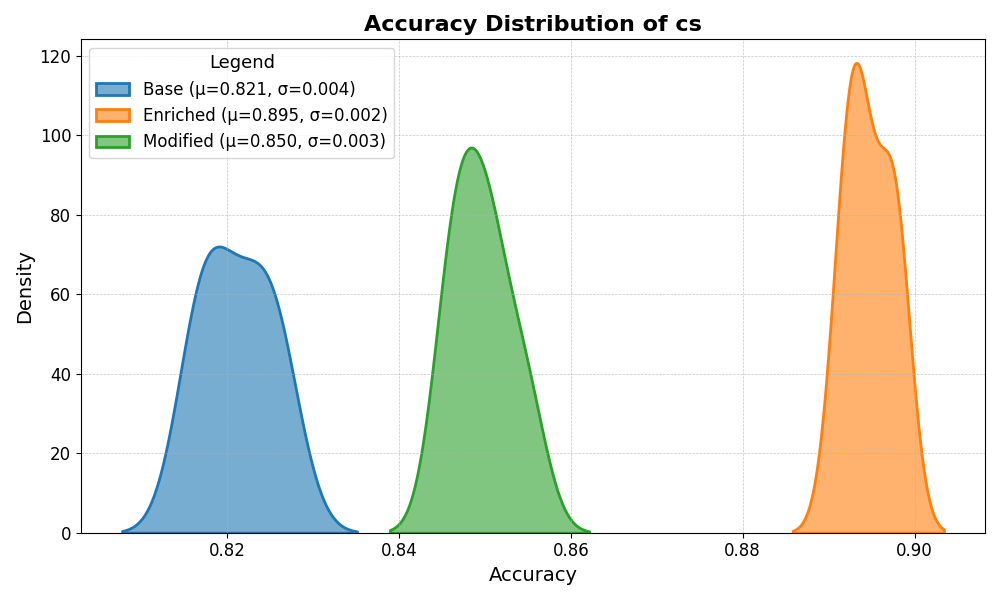
\includegraphics[width=0.9\textwidth]{gfx/cs_accuracy.png}
    \caption{Distribution of accuracy values for the base, enriched, and modified models on the \textit{cancer screening (cs)} event log.
    The plot illustrates kernel density estimates of accuracy, with shaded regions representing the distribution spread.}
    \label{fig:cs_accuracy}
\end{figure}

\textit{Age} influences whether issues are detected during screening,
as patients over the age of 60 have a 70\% probability of proceeding to \textit{explain diagnosis}
and a 30\% probability of \textit{inform prevention},
whereas those probabilities are reversed for patients aged 60 or younger.
\textit{Gender} directly determines whether a patient undergoes \textit{prostate screening} or \textit{mammary screening},
with probabilities of 100\% or 0\% respectively.
Since these distinctions are medically justified, no fairness correction is necessary so far.  

However, \textit{gender} also introduces an unfair bias when assessing eligibility,
where male patients have a 70\% likelihood of being accepted into \textit{collect history}
and a 30\% likelihood of being sent to \textit{refuse screening},
while for female patients, these probabilities are reversed.
Therefore, when evaluating the fairness of our models,
we calculate $\Delta \textit{DP}$ for the positive outcome
\textit{collect history} between male and female patients for samples with the previous activity \textit{assess eligibility}.

\begin{figure}[h!]
    \centering
    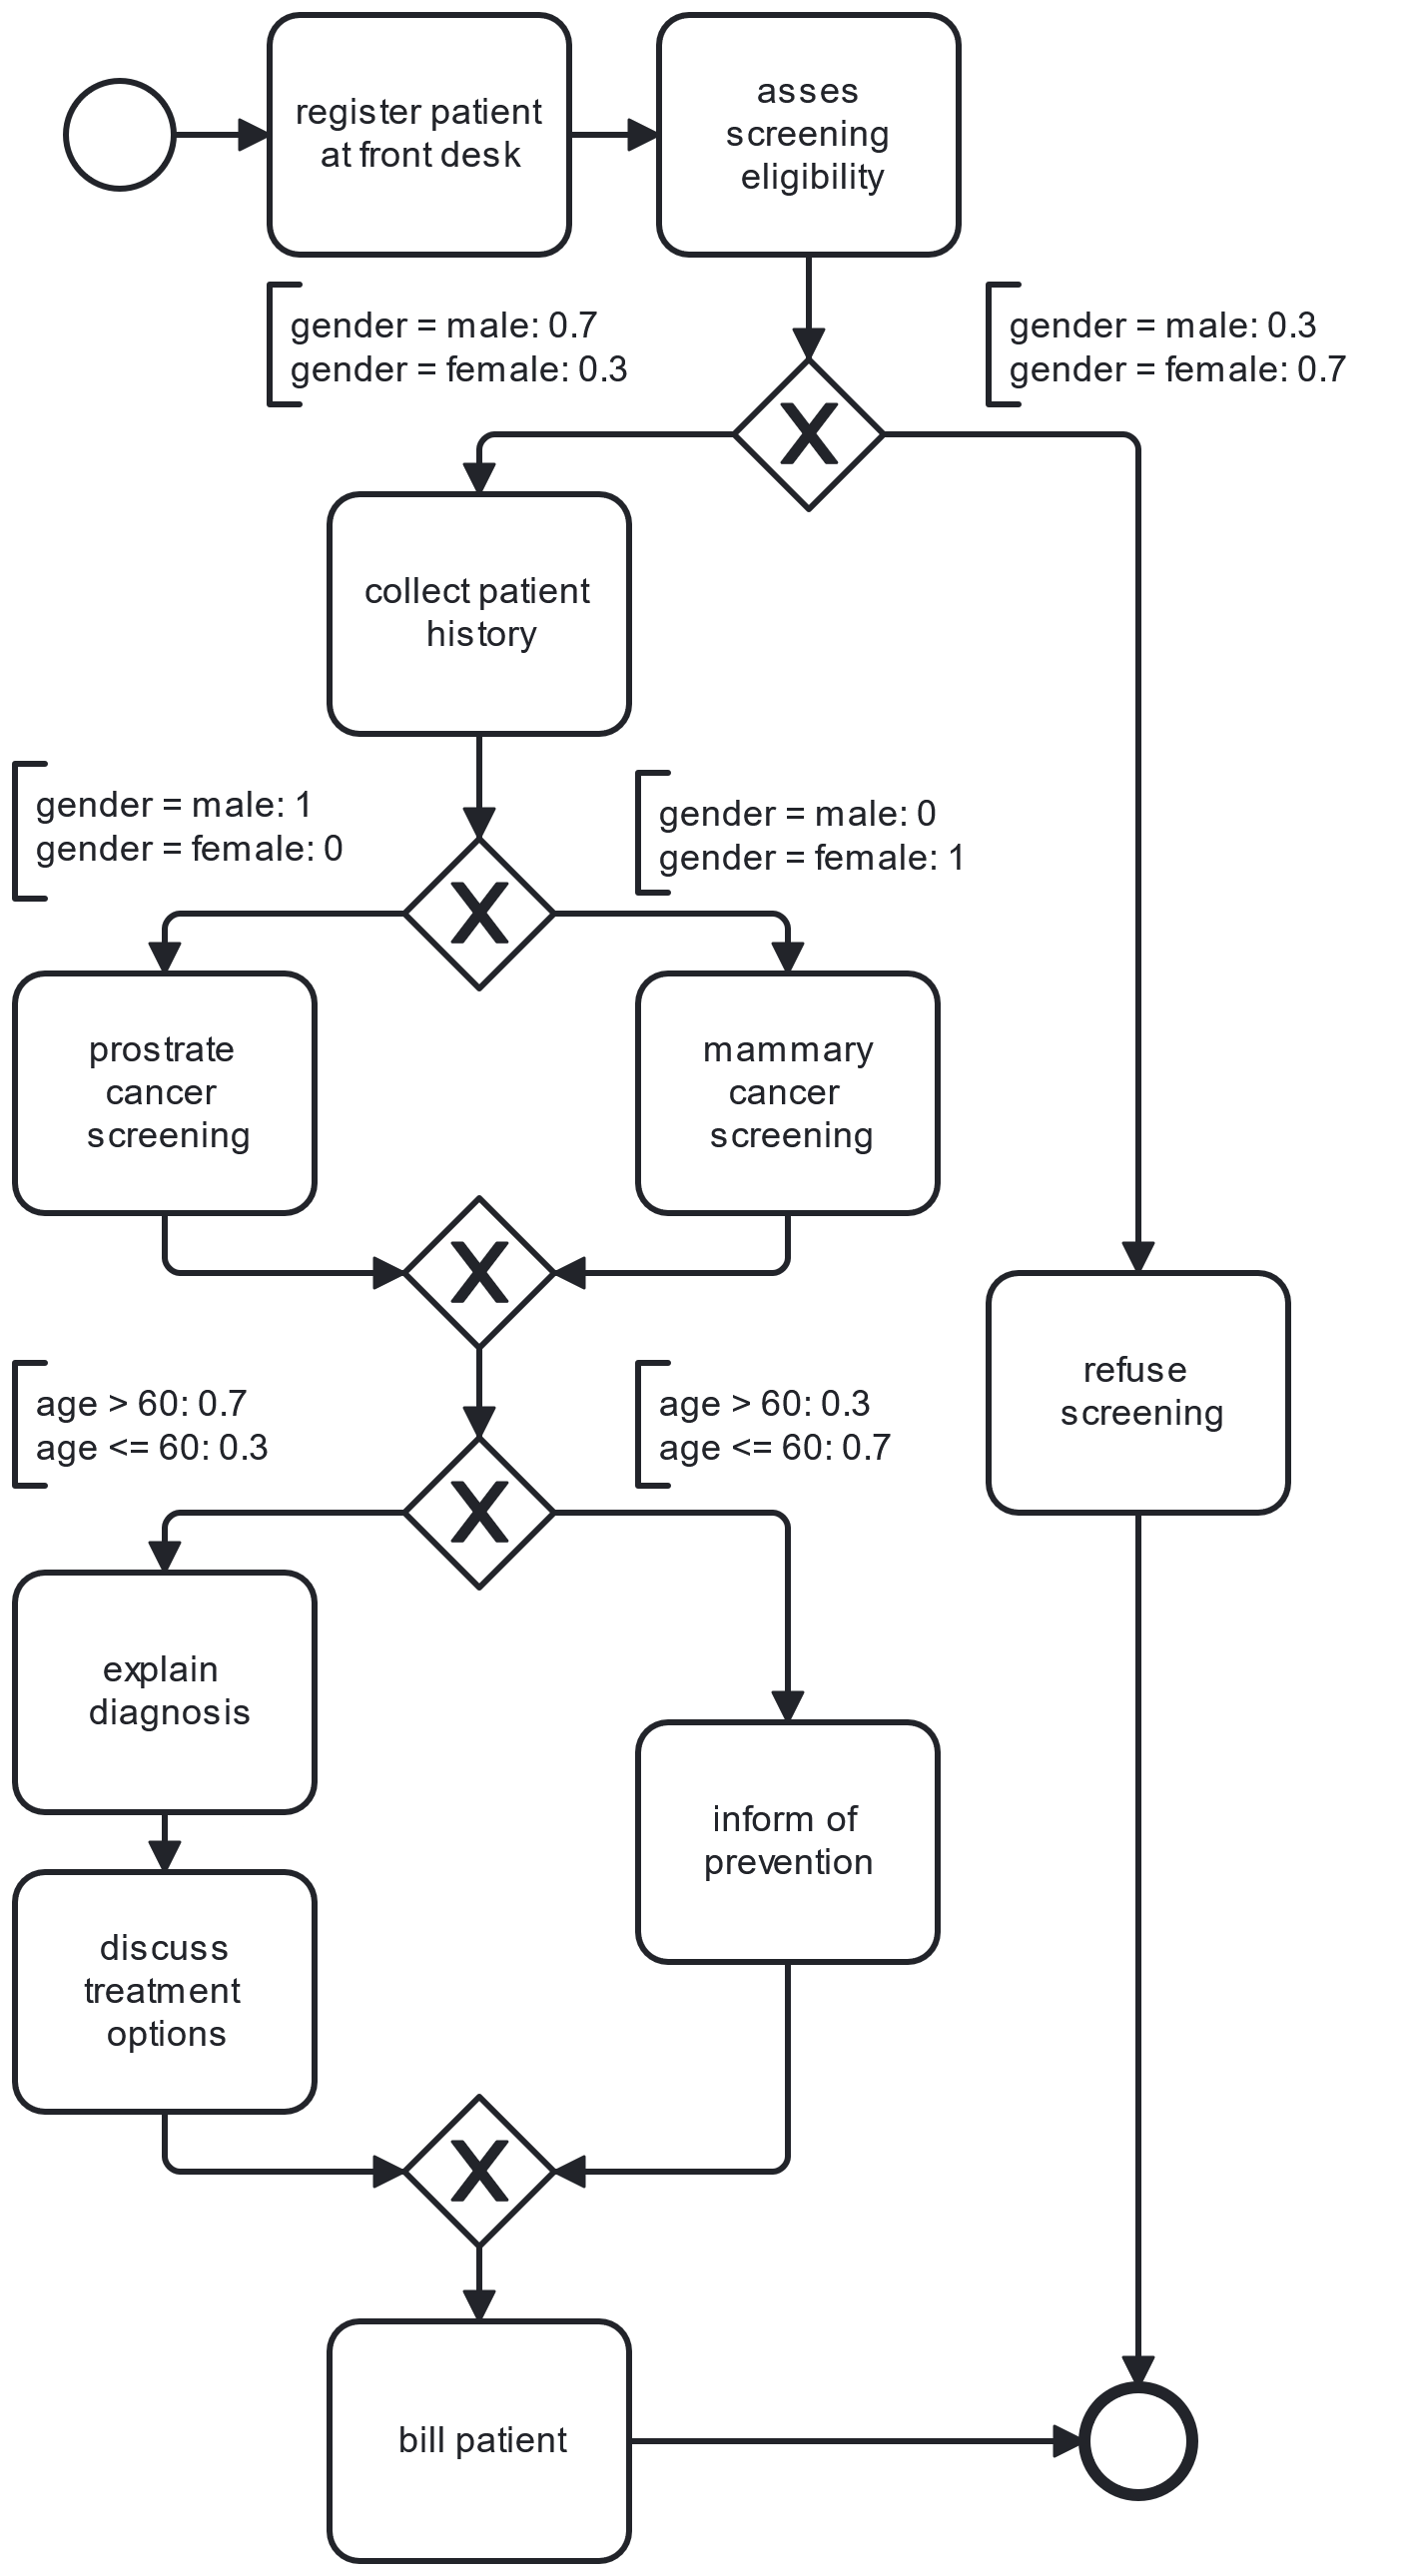
\includegraphics[width=\textwidth,height=0.7\textheight,keepaspectratio]{gfx/cancer_screening.png}
    \caption{This figure shows the BPMN diagram of the process model used for simulating the \textit{cancer screening} event log.
            The branches of the gateways are annotated with the underlying conditions based on the case attribute values and their corresponding probabilities.}
    \label{fig:cancer_screening}
\end{figure}

\section{Hospital Billing}
The \textbf{Hospital Billing} \cite{hospital_billing} event log
is a widely recognized dataset in process mining and healthcare analytics.
Extracted from the financial modules of a hospital's ERP system,
this event log records the sequence of activities involved in billing medical services.
The dataset comprises 100,000 cases, representing a randomly selected sample of process instances recorded over three years.
It includes a total of 17 distinct activities, capturing various steps in the billing workflow.  

To optimize computational efficiency for both training and testing,
we follow the approach in \cite{fairness_foundation} and use only the last 20,000 cases.
It is important to note that events and attribute values have been anonymized to ensure confidentiality.
For this purpose, the timestamps have been randomized as well,
with only the relative time intervals between events within a case preserved.
As a result, the last 20,000 cases do not necessarily correspond to the most recent process instances.  

Unfortunately, the event log doesn't contain any case attributes we can use for our experiments.
Therefore, we will enrich the data with the numerical case attribute \textit{age}
and the categorical attribute \textit{gender}.
For this event log, we consider both of these attributes to be sensitive.
A preliminary analysis of the \textbf{Directly-Follows Graph (DFG)},
a process model representation that captures transitions between activities,
reveals relatively few decision points where bias could be introduced.
However, two key points in the process stand out:  
\begin{itemize}  
    \item Whether a case includes the activity \textit{CHANGE DIAGN}, indicating a modification in the assigned diagnosis.  
    \item Whether, after the \textit{RELEASE} activity, the case transitions to \textit{CODE OK} or \textit{CODE NOK},
    where \textit{CODE OK} signifies successful billing, while \textit{CODE NOK} indicates a rejected or problematic case.  
\end{itemize}  
Since changes in diagnosis may be medically justified,
we do not consider biases related to \textit{CHANGE DIAGN} as problematic.
However, demographic disparities in the assignment of \textit{CODE OK} and \textit{CODE NOK} raise fairness concerns.
Given the relatively small number of cases that transition to \textit{CODE NOK},
the artificially embedded biases in age and gender must be strong enough to create a measurable disparity in the enriched model.  

\begin{figure}[h!]
    \centering
    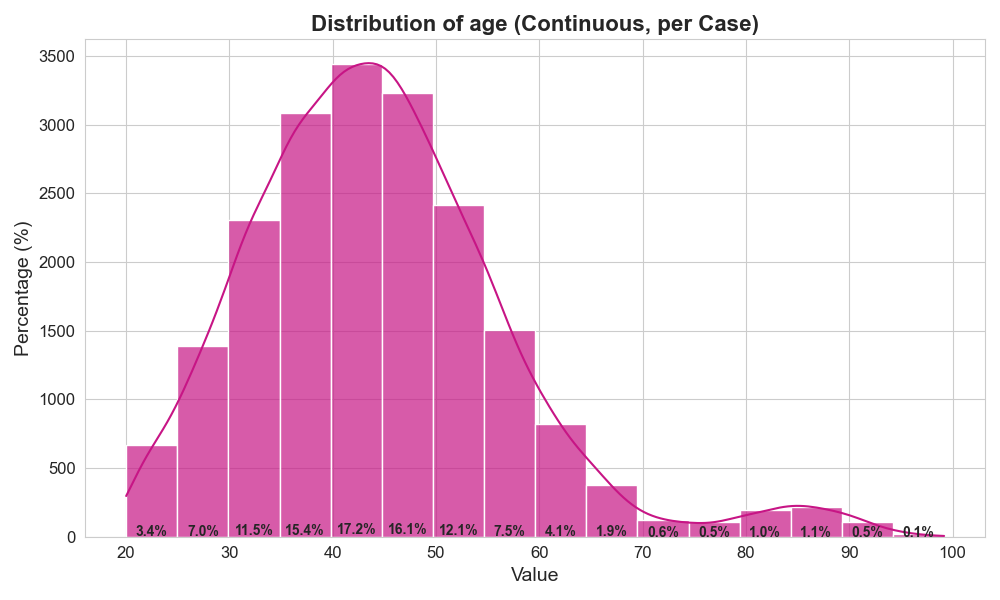
\includegraphics[width=0.9\textwidth]{gfx/hb_age.png}
    \caption{The distribution of the attribute \textit{age},
    when it causes bias in the \textit{hospital billing} event log.}
    \label{fig:hb_age}
\end{figure}

We create four experimental conditions by considering all possible combinations of bias and no bias
for the enriched attributes \textit{age} and \textit{gender}.
This setup enables us to evaluate how each biased attribute individually, as well as in combination,
influences the fairness of the process.  
If \textit{age} does not introduce bias, it follows a normal distribution with a mean of 50,
a standard deviation of 15, and is constrained between 20 and 100.
If \textit{gender} does not introduce bias, it is distributed as 49.5\% \textit{male}, 49.5\% \textit{female}, and 1\% \textit{non-conforming}.  
If \textit{age} causes bias, the assignment follows these probabilistic rules:
\begin{itemize}  
    \item \textbf{If} the event sequence contains \textit{CODE NOK},
        \textbf{then} age follows a normal distribution with mean 85, standard deviation 5, and is limited between 20 and 100.  
    \item \textbf{Else if} the event sequence contains \textit{CHANGE DIAGN},
        \textbf{then} age follows a normal distribution with mean 50, standard deviation 10, and is limited between 20 and 85.  
    \item \textbf{Else} (if none of the above conditions apply),
        \textbf{then} age follows a normal distribution with mean 40, standard deviation 10, and is limited between 20 and 85.  
\end{itemize}  
The resulting distribution is visualized in Figure \ref{fig:hb_age}.
And if \textit{gender} causes bias, the probabilistic rules are:
\begin{itemize}  
    \item \textbf{If} the event sequence contains \textit{CODE NOK},
        \textbf{then} \textit{male}: 10\%, \textit{female}: 10\%, \textit{non conforming}: 80\%.  
    \item \textbf{Else if} the event sequence contains \textit{CHANGE DIAGN},
        \textbf{then} \textit{male}: 29.5\%, \textit{female}: 69.5\%, \textit{non conforming}: 1\%.  
    \item \textbf{Else} (if none of the above conditions apply),
        \textbf{then} \textit{male}: 69.95\%, \textit{female}: 29.95\%, \textit{non conforming}: 0.1\%.  
\end{itemize}  
These rules result in an assigment of around 55.8\% male, 41.4\% female and 2.8\% non-conforming patients.

\begin{figure}[h!]
    \centering
    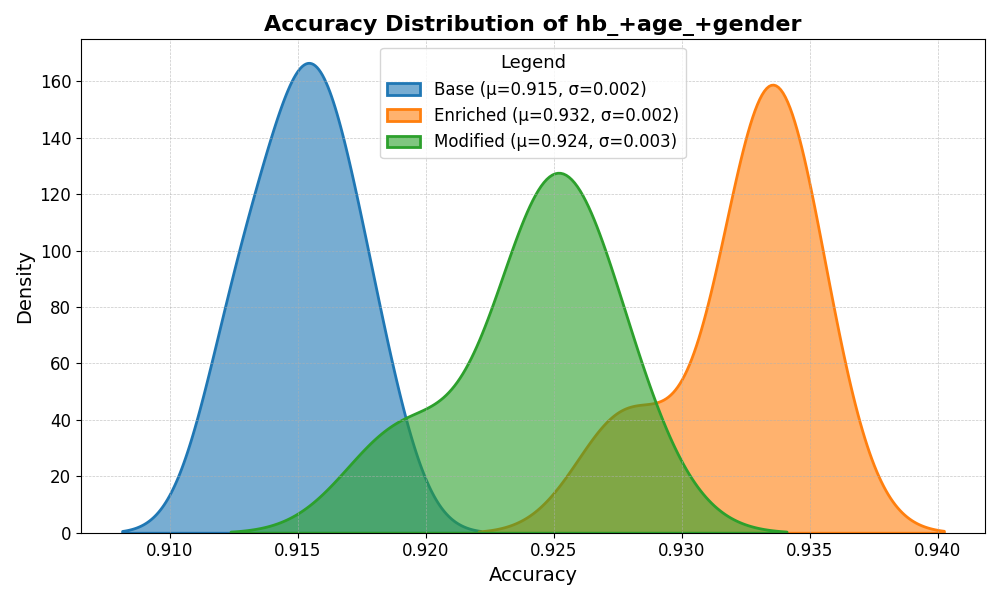
\includegraphics[width=0.9\textwidth]{gfx/hb_accuracy.png}
    \caption{Distribution of accuracy values for the base, enriched, and modified models on the \textit{hospital billing} event log,
    where both \textit{age} and \textit{gender} cause bias \textit{(hb\_+age\_+gender)}.
    The plot illustrates kernel density estimates of accuracy, with shaded regions representing the distribution spread.}
    \label{fig:hb_accuracy}
\end{figure}

To assess fairness, we measure \(\Delta \textit{DP}\) at the decision point following \textit{RELEASE},
where \textit{CODE OK} is considered the positive outcome.
Since \textit{gender} includes three categories,
we evaluate \(\Delta \textit{DP}\) for the split into \textit{gender-conforming} individuals (\textit{male} and \textit{female})
and \textit{non-conforming} individuals.
For \textit{age}, we split the group into patients are 85 or older versus those younger than 85.

\begin{table}[h!]
    \centering
    \scriptsize
    \renewcommand{\arraystretch}{1.2}
    \setlength{\tabcolsep}{6pt}
    \begin{tabular}{>{\centering\arraybackslash}m{1.9cm} | ccc}
        \toprule
        \makecell{\textbf{Event Log}\\[1ex]} & \multicolumn{3}{c}{\textbf{Accuracy}} \\
        & Base & Modified & Enriched \\
        \midrule
        -age, -gender &  .915 $\pm$ .003 &  .916 $\pm$ .002 &  .916 $\pm$ .002 \\
        -age, +gender &  .915 $\pm$ .003 &  .921 $\pm$ .002 &  .926 $\pm$ .002 \\
        +age, -gender &  .915 $\pm$ .003 &  .918 $\pm$ .005 &  .928 $\pm$ .005 \\
        +age, +gender &  .915 $\pm$ .003 &  .924 $\pm$ .003 &  .932 $\pm$ .002 \\
        \bottomrule
    \end{tabular}

    \vspace{0.3cm}

    \begin{tabularx}{\textwidth}{>{\centering\arraybackslash}m{1.9cm} | ccc | ccc}
        \toprule
        \makecell{\textbf{Event Log}\\[1ex]} & \multicolumn{3}{c|}{\textbf{Demographic Parity (Age)}} & \multicolumn{3}{c}{\textbf{Demographic Parity (Gender)}} \\
        & Base & Modified & Enriched & Base & Modified & Enriched \\
        \midrule
        -age, -gender &  .007 $\pm$ .004 &  .006 $\pm$ .002 &  .006 $\pm$ .002 &  .007 $\pm$ .004 &  .013 $\pm$ .014 &  .013 $\pm$ .014 \\
        -age, +gender &  .009 $\pm$ .005 &  .014 $\pm$ .022 &  .044 $\pm$ .008 &  .014 $\pm$ .013 &  .110 $\pm$ .168 &  .840 $\pm$ .036 \\
        +age, -gender &  .012 $\pm$ .011 &  .015 $\pm$ .023 &  .891 $\pm$ .023 &  .006 $\pm$ .002 &  .006 $\pm$ .004 &  .084 $\pm$ .029 \\
        +age, +gender &  .015 $\pm$ .011 &  .068 $\pm$ .119 &  .921 $\pm$ .028 &  .012 $\pm$ .010 &  .069 $\pm$ .122 &  .832 $\pm$ .039 \\
        \bottomrule
    \end{tabularx}
    \vspace{0.2cm}
    \caption{Evaluation of accuracy and demographic parity for the four versions of the \textit{Hospital Billing} log.
    The attributes \textit{age} and \textit{gender} are annotated based on whether they introduce a bias (+) or not (-).
    The reported values represent the mean ($\mu$) and standard deviation ($\sigma$) across validation folds, expressed as $\mu \pm \sigma$.}
    \label{tab:hb_combined}
\end{table}

%TODO: DFG

\section{BPI Challenge 2012}
The \textbf{BPI Challenge 2012} \cite{bpi_2012} event log, consisting of 13,087 cases, is a well-known dataset in process mining,
sourced from a Dutch financial institution.
It captures multiple subprocesses within a loan application procedure, each distinguished by specific prefixes.
These subprocesses include application states, denoted by the \textit{A\_} prefix, offer states, represented by the \textit{O\_} prefix,
and work items, labeled with the \textit{W\_} prefix.

For our analysis, we focus specifically on the \textit{A\_} subprocess, which pertains to the application phase of the loan procedure.
This subprocess is particularly relevant for examining fairness concerns,
as it involves crucial decision points that influence applicants' outcomes.
Within this subprocess, there are 10 distinct event types,
capturing key activities such as application submission, assessment, approval, and rejection.
Although the event log doesn't contain any sensitive case attributes,
the attribute \textit{AMOUNT\_REQ} specifies the amount of loan requested by the customer.
Since the amount is crucial information for deciding whether an application should be accepted,
we consider it to be a non-sensitive case attribute, which can also be utilized by the fair Base Model.

In order to explore our fairness problem statement, we enrich the event log with the sensitive categorical case attribute \textit{gender}.
To explore fairness concerns, we enrich the event log with the categorical sensitive case attribute \textit{gender}.
The DFG highlights two key decision points where biases could be introduced:
\begin{itemize}
\item Whether an application transitions to \textit{A\_PREACCEPTED} or \textit{A\_DECLINED} after \textit{A\_PARTLYSUBMITTED}.
\item Which activity follows after \textit{A\_FINALIZED},
with the most common options being either \textit{A\_APPROVED} or \textit{A\_CANCELLED}.
\end{itemize}
Therefore, we choose the assigment rules for \textit{gender} are as follows:
\begin{itemize}  
    \setlength{\itemsep}{0pt}
    \item \textbf{If} the event sequence contains \textit{A\_APPROVED},
        \textbf{then} \textit{female}: 70\%, \textit{male}: 30\%.  
    \item \textbf{Else if} the event sequence contains \textit{A\_CANCELLED},
        \textbf{then} \textit{female}: 30\%, \textit{male}: 70\%.  
    \item \textbf{Else if} the event sequence contains \textit{A\_PARTLYSUBMITTED} followed by \textit{A\_PRE\-ACCEPTED},
        \textbf{then} \textit{female}: 70\%, \textit{male}: 30\%.  
    \item \textbf{Else if} the event sequence contains \textit{A\_PARTLYSUBMITTED} followed by \textit{A\_DE\-CLINED},
        \textbf{then} \textit{female}: 30\%, \textit{male}: 70\%.  
    \item \textbf{Else} (if none of the above conditions apply),
        \textbf{then} \textit{female}: 50\%, \textit{male}: 50\%.  
\end{itemize}  
These rules result in around 56.6\% male and 43.4\% female applicants.

In the context of this event log, we only consider demographic disparities at decision of whether an application transitions to
\textit{A\_PREACCEPTED} or \textit{A\_DECLINED} to be unfair.
Thus, we measure $\Delta \textit{DP}$ for samples with the previous activity \textit{A\_PARTLYSUBMITTED},
considering \textit{A\_PREACCEPTED} as the positive outcome.
Since \textit{gender} is binary in this dataset,
we compare its impact on the probability of \textit{A\_PREACCEPTED} between \textit{male} and \textit{female} applicants.

\begin{figure}[h!]
    \centering
    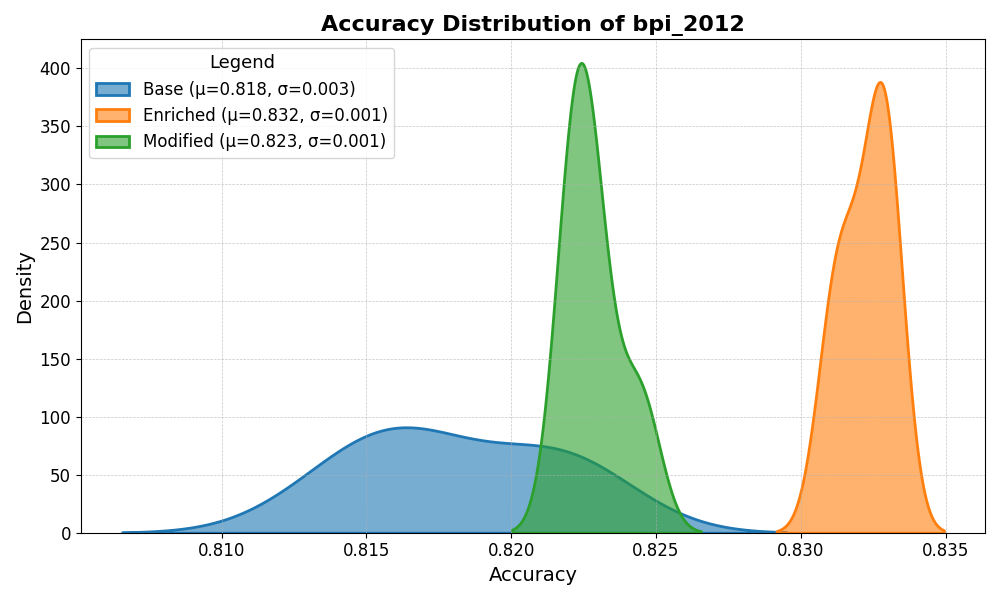
\includegraphics[width=0.9\textwidth]{gfx/bpi_2012_accuracy.png}
    \caption{Distribution of accuracy values for the base, enriched,
    and modified models on the \textit{BPI Challenge 2012 (bpi\_2012)} event log.
    The plot illustrates kernel density estimates of accuracy, with shaded regions representing the distribution spread.}
    \label{fig:bpi_accuracy}
\end{figure}

\begin{table}[h!]
    \centering
    \scriptsize
    \renewcommand{\arraystretch}{1.2}
    \setlength{\tabcolsep}{6pt}
    \begin{tabularx}{\textwidth}{>{\centering\arraybackslash}m{1.7cm} | ccc | ccc}
        \toprule
        \textbf{Event Log} & \multicolumn{3}{c|}{\textbf{Accuracy}} & \multicolumn{3}{c}{\textbf{Demographic Parity}} \\
        & Base & Modified & Enriched & Base & Modified & Enriched \\
        \midrule
        cs &  .821 $\pm$ .004 &  .850 $\pm$ .003 &  .895 $\pm$ .002 &  .001 $\pm$ .001 &  .013 $\pm$ .024 &  .999 $\pm$ .002 \\
        hb\_gender &  .915 $\pm$ .003 &  .921 $\pm$ .002 &  .926 $\pm$ .002 &  .014 $\pm$ .013 &  .110 $\pm$ .168 &  .840 $\pm$ .036 \\
        hb\_age &  .915 $\pm$ .003 &  .918 $\pm$ .005 &  .928 $\pm$ .005 &  .012 $\pm$ .011 &  .015 $\pm$ .023 &  .891 $\pm$ .023 \\
        bpi\_2012 &  .818 $\pm$ .003 &  .823 $\pm$ .001 &  .832 $\pm$ .001 &  .058 $\pm$ .019 &  .054 $\pm$ .014 &  .525 $\pm$ .036 \\
        \bottomrule
    \end{tabularx}
    \vspace{0.2cm} % adds a small space between the two tables
    \caption{Evaluation of accuracy and demographic parity for the \textit{cancer screening} log (cs),
    the \textit{BPI Challgenge 2012} log (bpi\_2012) and two versions of the \textit{Hospital Billing} log,
    where only the attribute \textit{age} introduces a bias (hb\_age) and only the attribute \textit{gender} introduces a bias (hb\_gender).
    The reported values represent the mean ($\mu$) and standard deviation ($\sigma$) across validation folds, expressed as $\mu \pm \sigma$.
    }
    \label{tab:evaluation_results}
\end{table}

%TODO: DFG

\section{Discussion}
% we will now discuss the results stemming from our experiments, as presented in tables \ref{tab:hb_combined} and \ref{tab:evaluation_results}

% cancer screening
    % due to its simulated nature and the very strong influence of the sensitive attributes, this event log has the most clear results
    % clear improvement in accuracy over baseline
    % delta DP is close to 0 for modified model, just as baseline

% bpi
    % difference in accuracy between models diminished,
    % since it's calculated over larger number of activities,
    % gender only influence few transitions, even then impact not as strong as in the cancer screening log
    % AMOUNT_REQ is also provided to base model, explains a lot of the transitions of application
    % very low standard deviation -> implies that results are significant nevertheless
    % would be bigger if the effect of the sensitive 
    % nevertheless, our methodology effectively reduces bias to the base level, while keeping accuracy higher than base level
    % not quite zero, possibly because of correlation gender with AMOUNT_REQ, influence not considered

% hospital billing
    % difference in accuracy minimal here as well, for similar reasons
    % even smaller, because the attributes have less impact
    % finally 4 different variations: see impact on behavior whether attribute is biased or not
    % both attributes not biased:
        % modified is identical to enriched, since no nodes needed to be removed
        % good, this means our methodology doesn't reduce accuracy when no unfairness present
    % one attribute biased:
        % similar to cancer screening
        % delta DP close to baseline, while better accuracy than baseline
    % both attributes biased:
        % enhances effect from one biased: even more accurate than baseline
        % delta DP heavily reduced for both attributes, compared to enriched model

% in conclusion:
%goal of finding a classifier that balances the accuracy of the enriched model and the fairness of the baseline model was successful